% ============================================================
%  main.tex — Elsevier CAS Double-Column (cas-dc)
%  Zero-Shot Consumer Financial Complaint Classification
%  Using Open-Source LLMs on an HPC Cluster
% ============================================================
\documentclass[a4paper,fleqn]{cas-dc}

\usepackage[numbers]{natbib}
\usepackage{amsmath,amssymb}
\usepackage{graphicx}
\usepackage{booktabs}
\usepackage{array}
\usepackage{url}
\usepackage{hyperref}
\usepackage{multirow}
\usepackage{xcolor}
\usepackage{microtype}
\usepackage{placeins}
\setlength{\emergencystretch}{2em}
\hfuzz=130pt
\renewcommand{\floatpagefraction}{0.85}
\renewcommand{\textfraction}{0.05}

\hypersetup{
  colorlinks=true,
  linkcolor=black,
  citecolor=black,
  urlcolor=black
}

% =============================================================
\begin{document}
\let\WriteBookmarks\relax
\def\floatpagepagefraction{1}
\def\textpagefraction{.001}

\shorttitle{Can Open-Source LLMs Replace Paid APIs for Zero-Shot Complaint Classification?}
\shortauthors{M.~Tan and H.~Bak{\i}r}

% ---- Title --------------------------------------------------
\title[mode=title]{Can Open-Source LLMs Replace Paid APIs for Zero-Shot Consumer Complaint Classification?}

% ---- Authors ------------------------------------------------
\author[1]{Muhammet Tan}[orcid=0009-0004-9430-372X]
\cormark[1]
\ead{muhammet.tan@sivas.edu.tr}
\credit{Conceptualization, Methodology, Software, Formal analysis,
        Writing -- Original Draft}

\affiliation[1]{organization={Department of Computer Engineering,
                Sivas University of Science and Technology},
                city={Sivas},
                postcode={58010},
                country={Turkey}}

\author[1]{Halit Bak{\i}r}
\credit{Supervision, Writing -- Review \& Editing, Resources}

\cortext[1]{Corresponding author}

% ---- Abstract -----------------------------------------------
\begin{abstract}
Automated classification of consumer financial complaints has significant
implications for regulatory oversight and customer service prioritisation.
While recent studies have demonstrated strong zero-shot performance using
large proprietary language model (LLM) APIs, those approaches incur
substantial and recurring monetary costs. In this paper we investigate
whether open-source, locally deployed LLMs can match the classification
quality of their paid-API counterparts with no commercial API expenditure. We benchmark
eleven open-weight models (six standard and five reasoning) on the
Consumer Financial Protection Bureau (CFPB) five-category zero-shot
task, across two experimental conditions (balanced and imbalanced),
three random seeds, and two narrative length limits (250 and 500
characters). Our best model, \texttt{gemma4:12b}, achieves a mean
weighted F1 of $0.774 \pm 0.016$ on the balanced evaluation ---
performance competitive with paid GPT-4.5 (F1~0.7763) and o1
(F1~0.7764) under a protocol-matched evaluation setting,
with no commercial API expenditure. Notably, this top result comes from a 12B standard
(non-reasoning) model, challenging the view that reasoning models are
necessary for structured classification tasks. We analyse off-label
prediction behaviour and provide deployment recommendations based on
the latency--accuracy trade-off observed across all eleven models.
\end{abstract}

% ---- Highlights (max 85 chars each) -------------------------
\begin{highlights}
\item Eleven open-source LLMs benchmarked on CFPB zero-shot classification at zero API cost
\item gemma4:12b achieves protocol-matched performance comparable to paid LLMs without commercial API expenditure
\item Standard models can match or surpass larger reasoning models on structured classification
\item Imbalanced evaluation reveals majority-class bias in aggregate accuracy metrics
\item Reproducible HPC pipeline enables local LLM deployment without third-party APIs
\end{highlights}

% ---- Keywords -----------------------------------------------
\begin{keywords}
consumer complaint classification \sep
large language models \sep
zero-shot learning \sep
open-source LLMs \sep
CFPB \sep
reasoning models \sep
natural language processing
\end{keywords}

\maketitle

% =============================================================
\section{Introduction}
\label{sec:intro}

The Consumer Financial Protection Bureau (CFPB) publishes a public
database of consumer complaints submitted against financial institutions
in the United States. The dataset spans dozens of product categories
and hundreds of thousands of narratives, making it one of the most
accessible and practically relevant corpora for natural language
processing (NLP) research in the financial domain. Accurately routing
and categorising these complaints has direct implications for
regulatory efficiency, bank compliance teams, and consumer advocacy
organisations: a miscategorised complaint may be forwarded to the wrong
department, delayed, or deprioritised
\cite{das2024explainable,liu2024framework,jondhale2024cfpb}.

Unlike many benchmark text-classification datasets, consumer complaint
narratives are not merely short topic labels embedded in clean prose.
They often contain informal descriptions of stressful financial events,
institution names, dates, partial account details, and overlapping
product issues. A single complaint may mention credit reporting, debt
collection, and a credit card dispute in the same narrative, while the
supervised label assigns only one product category. This ambiguity makes
the task more realistic than many standard NLP benchmarks and also more
valuable as a test bed for instruction-following models: a useful system
must map noisy, human-written narratives to a constrained regulatory
taxonomy without inventing new labels.

The practical motivation is equally strong. Complaint triage is a
high-volume activity in which automation can reduce manual screening
time, support earlier detection of recurring institutional problems,
and provide consistent first-pass routing \cite{di2023complaint}.
At the same time, financial complaint text is operationally sensitive
in a deeper sense than cost alone. Banks, regulators, and supervisory
authorities operate under overlapping data-governance frameworks:
the General Data Protection Regulation \cite{gdpr2016} and the EU AI
Act \cite{euaiact2024} may legally restrict the transfer of personal
financial data to third-party services outside an institution's control;
the European Banking Authority's Guidelines on Outsourcing Arrangements
\cite{eba2019outsourcing} additionally require financial institutions to
conduct rigorous risk assessments, maintain supervisory access rights, and
ensure data confidentiality for any critical function outsourced to a cloud
provider. Taken together, these frameworks impose significant compliance
burdens on API-based deployments and may, in many institutional contexts,
effectively preclude them. A classification pipeline that depends on
external API calls is therefore not merely more expensive, but potentially
non-compliant. This makes local inference, on-premises data residency, and
reproducible infrastructure more than cost-reduction measures; they are
\emph{prerequisites for compliant deployment} in regulated environments
and form a central part of the methodological problem this paper addresses.

Traditional approaches to complaint classification relied on
bag-of-words representations, support vector machines, and logistic
regression. The emergence of BERT \cite{devlin2019bert} and its
domain-adapted successors marked a step change, enabling much richer
semantic representations and pushing classification accuracy above
90\,\% in fine-tuned settings \cite{vairetti2024bert}. More recently,
the advent of instruction-following LLMs such as GPT-3 \cite{brown2020gpt3}
and its successors opened the possibility of \emph{zero-shot}
classification: a model is simply given the candidate categories in
a prompt and is asked to assign the most appropriate one, requiring
no task-specific training data at all
\cite{kojima2022zeroshotcot,madanchian2024genai}.

For consumer complaint analysis, this zero-shot setting is attractive
because financial taxonomies evolve and labelled data may be costly to
curate for every new jurisdiction, product definition, or institutional
workflow. However, zero-shot classification also shifts the main
engineering burden from model training to prompt adherence, output
parsing, and deployment cost. A model that returns a plausible but
unsupported category such as \texttt{credit\_collection} may look
linguistically competent while still failing the regulatory routing
task. Therefore, evaluating off-label behaviour is essential alongside
accuracy and F1.

Roumeliotis~et~al.\ \cite{roumeliotis2025think} conducted a
comprehensive zero-shot benchmark of 14 state-of-the-art proprietary
and commercial models --- including GPT-4o, GPT-4.5, Claude~3.5/3.7,
Gemini~2.0, o1, o3-mini, and DeepSeek (API) --- on the same CFPB
dataset and five-category task. They reported that the best model,
OpenAI's o1, achieved an accuracy of 0.777 and an F1 of 0.7764, at a
cost of \$24.24 per thousand predictions. Their study provided strong
evidence that reasoning-enabled LLMs can outperform standard chat
models on this structured classification task. However, a critical
limitation of their work is that \emph{every} model was accessed
through a paid commercial API, creating a barrier to reproduction
and deployment in low-budget or data-sensitive environments.

This leaves an important open question: can open-weight models, served
locally on shared research infrastructure, deliver competitive
zero-shot complaint classification without API access? The answer is
not obvious. Smaller local models are cheaper to run but may be weaker
at following strict JSON-style instructions. Reasoning models may
improve disambiguation and output discipline, but they also generate
longer traces and increase latency. In addition, prior balanced
benchmarks do not show whether the same ranking survives under the
natural class imbalance of the CFPB corpus, where a majority
\texttt{credit\_reporting} class can inflate aggregate metrics.

The present paper addresses this gap directly. Our contributions are:

\begin{enumerate}
  \item To the best of our knowledge, we provide the first
        deployment-oriented benchmark of open-weight LLMs on the
        CFPB five-category zero-shot task, evaluating eleven models ---
        \texttt{gemma2:9b}, \texttt{gemma4:12b}, \texttt{mistral:7b},
        \texttt{mistral-nemo:12b}, \texttt{llama3.1:8b}, \texttt{phi4:14b},
        \texttt{deepseek-r1:8b}, \texttt{deepseek-r1:14b},
        \texttt{qwen3:8b}, \texttt{qwen3:14b}, and \texttt{gpt-oss:20b}
        --- at \textbf{zero API cost} on shared HPC infrastructure.
        The model set includes matched 12--14B variants per architecture
        family, enabling controlled cross-scale comparison.

  \item We document a complete, reproducible inference pipeline on the
        TRUBA ARF HPC cluster using Ollama and SLURM, including
        all deployment parameters needed to replicate our results.

  \item We conduct a second experiment using the natural (imbalanced)
        class distribution, evaluating whether performance patterns
        observed under artificial balance hold in a more realistic
        scenario.

  \item We provide a direct quantitative comparison with the paid-API
        results of Roumeliotis~et~al.\ \cite{roumeliotis2025think},
        showing that our best open-source model exceeds the reported
        GPT-4o score under the same evaluation protocol and remains
        competitive with more expensive API-based alternatives.

  \item We analyse off-label prediction behaviour --- instances where
        models invent labels outside the five prescribed categories ---
        as a proxy for instruction-following reliability.
\end{enumerate}

The remainder of this paper is structured as follows.
Section~\ref{sec:related} surveys the related literature.
Section~\ref{sec:data} describes the dataset and preprocessing
pipeline. Section~\ref{sec:setup} details the experimental setup.
Section~\ref{sec:results} presents results for both experiments.
Section~\ref{sec:discussion} discusses the findings.
Section~\ref{sec:conclusion} concludes with directions for future work.


% =============================================================
\section{Related Work}
\label{sec:related}

\subsection{From Rule-Based Systems to Transformer Models}

The challenge of automatically classifying consumer complaints has a
rich history that mirrors the broader trajectory of NLP research. Early
systems relied on keyword matching and hand-crafted feature engineering
paired with classical classifiers such as support vector machines and
na{\"i}ve Bayes. While effective for narrow, well-defined complaint
taxonomies, these approaches proved brittle in the face of the
linguistic diversity found in real-world financial complaint corpora
\cite{raju2022bertopic,jondhale2024cfpb}.
Lilleberg~et~al.\ \cite{lilleberg2015word2vec} demonstrated that pairing
support vector machines with Word2Vec embeddings improves text classification
over purely bag-of-words features, yet even these enriched representations
required domain-specific engineering and large labelled corpora.

The introduction of BERT \cite{devlin2019bert} triggered a significant
paradigm shift. Contextual word embeddings, obtained by pre-training on
large general-domain corpora and then fine-tuning on downstream tasks,
dramatically reduced the gap between human and machine performance on
text classification. Raju~et~al.\ \cite{raju2022bertopic} applied
BERTopic \cite{grootendorst2020bertopic}, FinBERT, DistilBERT, and
RoBERTa to a corpus of 684,653 CFPB complaints, demonstrating that
transformer-based topic models could discover latent complaint themes
without manual annotation. Vairetti~et~al.\ \cite{vairetti2024bert}
used the Spanish BERT variant BETO for complaint prioritisation,
achieving 92.1\,\% accuracy, illustrating that the BERT paradigm
transfers well across languages and regulatory contexts. Das~et~al.\
\cite{das2024explainable} pushed further by coupling transformer-based
classifiers with explainability techniques, enabling practitioners to
understand \emph{why} a complaint was assigned a given category --- a
requirement for regulatory compliance. Liu~et~al.\ \cite{liu2024framework}
proposed a structured LLM-based categorisation framework (CCF) with
real-time monitoring, demonstrating that modern LLMs can serve as
end-to-end complaint classification pipelines with minimal domain
customisation.

\subsection{The LLM Era and the Zero-Shot Paradigm}

The release of GPT-3 \cite{brown2020gpt3} introduced the few-shot and
zero-shot paradigms, in which a large pre-trained language model can
perform novel tasks from a natural language description alone. This
capability fundamentally changed the cost calculus of NLP system
development: instead of collecting thousands of labelled examples and
retraining a model, practitioners could now describe a task in a
prompt and obtain reasonable predictions immediately. Zhao~et~al.\
\cite{zhao2023survey} provide a comprehensive survey of the capabilities
and limitations of modern LLMs, noting that instruction-following
performance scales strongly with model size and training quality.

In the financial complaint domain, Correa~et~al.\ \cite{correa2024genai}
demonstrated that generative AI can simultaneously classify, summarise,
and draft responses to CFPB complaints, achieving 88\,\% classification
accuracy in a zero-shot setting. This result was notable because it
required no fine-tuning whatsoever, confirming that the rich language
representations encoded in large-scale pre-training are sufficient for
this task. Extending the zero-shot paradigm to service industries,
Roumeliotis~et~al.\ \cite{roumeliotis2024tourism} compared GPT-4 Omni
and BERT for customer review classification in tourism, finding that
GPT-4o achieved 67\,\% accuracy in a zero-shot setting versus 60.6\,\%
for fine-tuned BERT --- an early indication that zero-shot LLMs can
challenge fine-tuned specialised models.
In a related e-commerce study, Roumeliotis~et~al.\ \cite{roumeliotis2024ecommerce}
compared GPT-3.5 and LLaMA-2 alongside BERT and RoBERTa for product review
sentiment classification, confirming that LLMs achieve competitive performance
across diverse consumer feedback domains both before and after fine-tuning.
Li~et~al.\
\cite{li2024customerservice} further showed, through a comprehensive
customer service benchmark (TeleEval-CS), that fine-tuned open-source
LLMs can match proprietary counterparts when evaluated on
domain-specific dialogue tasks, motivating our investigation of
open-weight models.

A practically important contextual finding is that the CFPB complaint
corpus itself is changing. Shin~et~al.\ \cite{shin2025llmwritten}
analysed over 1.1 million CFPB complaints and found that approximately
9.8\,\% of complaints submitted after the public release of ChatGPT
exhibit strong evidence of LLM assistance. Liang~et~al.\
\cite{liang2025cfpb} independently estimated that roughly 18\,\% of
recent complaints are LLM-assisted. These findings underscore the
increasing entanglement of generative AI and financial consumer
protection, making robust automated classification even more important.

\subsection{Reasoning Models and the State of the Art}

The most recent development in this space has been the introduction of
chain-of-thought reasoning models \cite{wei2022chainofthought}, which
generate intermediate reasoning steps before arriving at a final answer.
DeepSeek-AI \cite{deepseekllm2024} demonstrated that open-source models
trained with careful scaling laws can match GPT-3.5 tier performance,
establishing the viability of open-weight alternatives before the
reasoning model era. Building on this foundation, Guo~et~al.\
\cite{guo2025deepseekr1} introduced DeepSeek-R1, an open-weight model
trained via reinforcement learning to produce structured reasoning
traces, achieving performance competitive with proprietary frontier
models on a range of benchmarks. Similarly, the
Qwen3 series \cite{qwen2025qwen3} introduced an explicit thinking mode
that can be toggled per query.

Roumeliotis~et~al.\ \cite{roumeliotis2025think} brought this reasoning
paradigm directly to the complaint classification setting. Testing
14 models on a balanced sample of 1,000 CFPB complaints across five
categories, they found that o1 (0.777 accuracy, F1~0.7764) and
GPT-4.5 (0.774, F1~0.7763) outperformed their non-reasoning
counterparts, and that reasoning models as a class exhibited fewer
off-label predictions. Their study is the closest antecedent to the
present work and provides the benchmark against which our results
are measured.

Bulgakov and Turchin \cite{bulgakov2026deepseek} proposed a two-stage
framework combining a reasoning model with a lightweight logistic-regression
corrector for rare-event prediction in consumer service domains,
demonstrating that reasoning-enhanced inference can mitigate
prevalence-driven bias without task-specific fine-tuning. G{\"u}ll{\"u}~et~al.\
\cite{gullu2025llama} fine-tuned LLaMA-3.1-8B on the same five-category
CFPB task used in our study, reaching 89.99\,\% accuracy and
establishing an approximate fine-tuning performance ceiling for that
model family.

\subsection{The Open-Source Gap}

Despite these advances, a critical gap remains in the literature. Every
paper benchmarking LLMs on CFPB complaint classification has relied
either on paid commercial APIs or on fine-tuned models that require
substantial labelled training data. Neither approach is accessible to
practitioners operating under strict data-governance constraints,
limited budgets, or air-gapped computing environments. The present
paper fills this gap by restricting itself entirely to open-weight
models deployed locally on shared HPC infrastructure, thereby
demonstrating that competitive zero-shot complaint classification is
achievable without any API cost or proprietary model access.


% =============================================================
\section{Dataset and Preprocessing}
\label{sec:data}

\subsection{Data Source}

We use the CFPB Consumer Complaints dataset originally published by
Tiwari \cite{tiwari2021cfpb} on Kaggle, which is a processed subset
of the public CFPB Consumer Complaint Database. The dataset covers
complaints submitted between March~2020 and March~2021 and contains
three columns: an unnamed index, \texttt{product} (the category label),
and \texttt{narrative} (the free-text complaint). The raw file
comprises 162,421 records consolidated to five target product categories:
\texttt{retail\_banking}, \texttt{credit\_reporting},
\texttt{credit\_card}, \texttt{mortgages\_and\_loans}, and
\texttt{debt\_collection}. This is the same dataset and label set used
by Roumeliotis~et~al.\ \cite{roumeliotis2025think}, ensuring
direct comparability.

\subsection{Class Distribution}

The original data are heavily imbalanced. After removing records with
empty \texttt{product} or \texttt{narrative} fields (10 rows removed,
162,411 remaining) and discarding narratives exceeding 500 characters
(resulting in 103,915 usable records), the class distribution shifts
to: \texttt{credit\_reporting}~63.6\,\%,
\texttt{debt\_collection}~14.1\,\%,
\texttt{mortgages\_and\_loans}~7.7\,\%,
\texttt{credit\_card}~7.5\,\%, and
\texttt{retail\_banking}~7.1\,\%. Before the length filter, the same
five-category corpus contains 162,411 records with
\texttt{credit\_reporting} accounting for 56.1\,\% of the data.
Fig.~\ref{fig:class_dist} illustrates how this skew propagates into
the experimental subsets: the imbalanced condition retains the
dominant \texttt{credit\_reporting} class at 51.1\,\%, while the
balanced condition enforces equal class sizes of 200~samples each.
At $N{=}1{,}000$, a model that defaults to the majority class in the
imbalanced setting would achieve 51.1\,\% accuracy with zero
language understanding --- motivating the need to report both conditions
side by side.

\begin{figure*}[t]
  \centering
  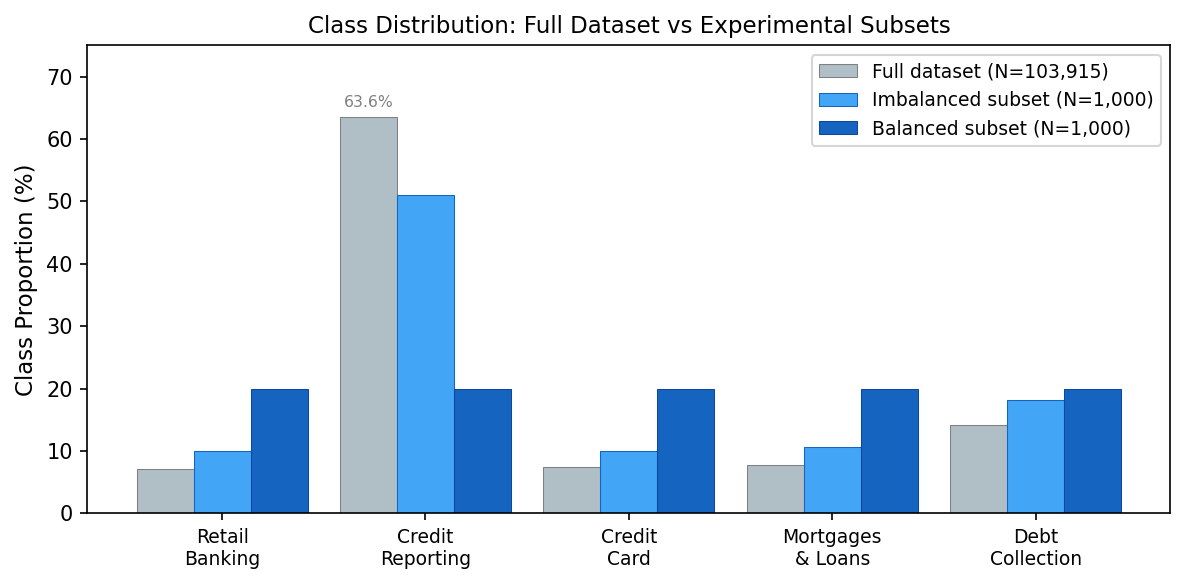
\includegraphics[width=0.78\textwidth]{figures/v2/class_distribution.png}
  \caption{Class proportions (\%) in the full post-filter dataset
           ($N{=}103{,}915$), the imbalanced experimental subset
           ($N{=}1{,}000$), and the balanced subset ($N{=}1{,}000$).
           In the imbalanced condition, \texttt{credit\_reporting}
           is still the dominant class at 51.1\,\%, confirming
           that balanced evaluation is essential to avoid
           majority-class inflation.}
  \label{fig:class_dist}
\end{figure*}

\subsection{Preprocessing Pipeline}

The preprocessing steps, implemented in Python using pandas, are applied
in the following order to every record:

\begin{enumerate}
  \item Drop rows with empty \texttt{product} or \texttt{narrative}.
  \item Retain only records belonging to the five target categories.
  \item Remove narratives longer than 500 characters, reducing processing
        time and GPU memory pressure while avoiding truncation artifacts
        during inference.
  \item Standardise narrative text: convert to lowercase, remove special
        characters, and normalise whitespace.
\end{enumerate}

\subsection{Experimental Subsets}

Two experimental conditions are defined, each evaluated under a
multi-seed, multi-size design to ensure statistically reliable estimates.

\textbf{Experiment~A (Balanced):} 200~records are sampled uniformly at
random from each of the five categories ($N=1{,}000$ total) using
stratified undersampling.
This follows the evaluation protocol of
Roumeliotis~et~al.\ \cite{roumeliotis2025think}.
All eleven open-source models in this study are evaluated on
\emph{exactly the same} complaint instances: a fixed random draw
controlled by a NumPy seed is used for every model within each
seed--size configuration, so every within-study comparison is
\emph{instance-identical}.
The cross-paper comparison with GPT-4.5 and o1 figures reported
by Roumeliotis~et~al.\ should be interpreted as protocol-matched
rather than instance-paired, because the reference paper does not
publish the exact sampled complaint identifiers.

{\sloppy
\textbf{Experiment~B (Imbalanced):} Records are sampled with proportions
reflecting the post-filter natural class distribution, subject to a
minimum of 100~samples per class. This yields $N{=}1{,}000$ with
\texttt{credit\_reporting}~51.1\,\%, \texttt{debt\_collection}~18.2\,\%,
\texttt{mortgages\_and\_loans}~10.7\,\%, \texttt{credit\_card}~10.0\,\%,
and \texttt{retail\_banking}~10.0\,\%.
The dominant \texttt{credit\_reporting} class means a naive majority
baseline would reach only 51.1\,\% accuracy with no language understanding.
\par}
This second experiment, absent from the closest antecedent benchmark,
assesses how class imbalance affects both accuracy estimates and
per-class performance patterns.

\textbf{Multi-seed and narrative-length design:}
Each condition is replicated with three independent random seeds (1, 2,
and 3) and at two narrative character-length limits (250 and 500
characters), yielding 12 datasets per model and 132 inference runs in
total (11~models $\times$~3~seeds~$\times$~2~conditions~$\times$~2~length
limits). All reported aggregate metrics and comparisons use the
500-character variant and are presented as mean~$\pm$~standard deviation
over the three seeds. The 250-character runs provide a narrative-length
sensitivity check discussed in Section~\ref{sec:sensitivity}.
This design addresses the single-seed limitation common in prior
zero-shot LLM benchmarks and allows us to distinguish robust ranking
patterns from seed-specific artefacts.

The choice of 250- and 500-character limits is motivated by the
narrative length distribution of the corpus. Fig.~\ref{fig:char_hist}
shows that the vast majority of usable narratives fall within the
0--500 character range across all three seeds, with the median near
250 characters. The two limits thus span the core of the distribution:
the 250-character variant tests performance on short narratives
(median length), while the 500-character variant includes the full
range of narratives up to the preprocessing cutoff.

\begin{figure*}[t]
  \centering
  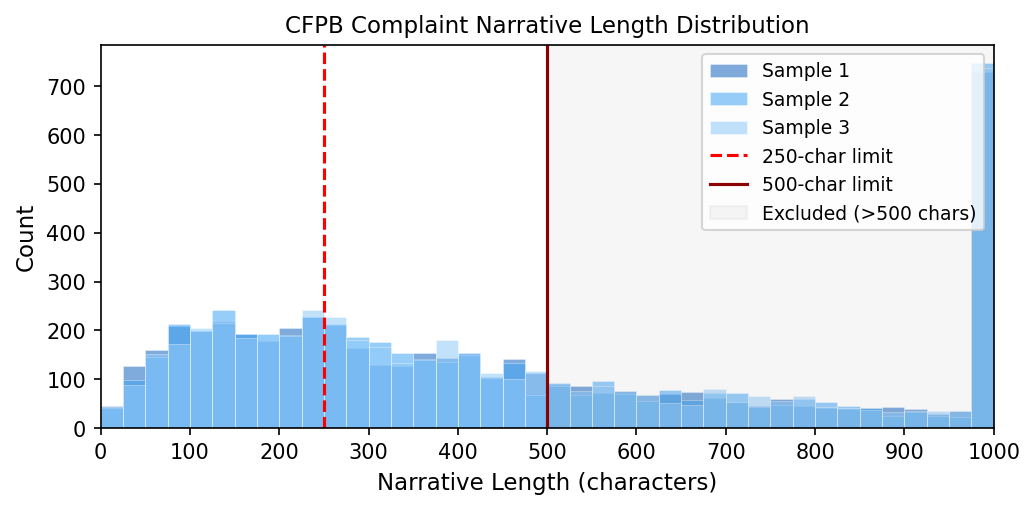
\includegraphics[width=0.78\textwidth]{figures/v2/char_length_histogram.png}
  \caption{Narrative character-length distribution across three balanced
           $N{=}1{,}000$ subsets (seeds 1--3, different colours).
           The dashed line marks the 250-character evaluation limit;
           the solid line marks 500 characters.
           Distributions are consistent across seeds, confirming
           reproducible sampling.}
  \label{fig:char_hist}
\end{figure*}


% =============================================================
\section{Experimental Setup}
\label{sec:setup}

\subsection{Infrastructure}

All inference experiments are conducted on the TRUBA ARF cluster,
the Turkish national high-performance computing facility. Jobs are
submitted via the SLURM scheduler to the \texttt{akya-cuda} partition.
Each job is allocated a single NVIDIA Tesla V100-SXM2-16\,GB GPU
(16\,GB VRAM), 10~CPU cores, and a 24-hour wall-clock time limit.
All models are pre-downloaded to the shared storage before job submission,
ensuring fully offline inference on compute nodes --- a configuration
that mirrors regulated or air-gapped deployment environments.

Model inference is handled by Ollama~v0.30.6, a self-contained
serving binary that manages model loading, KV-cache management,
and the REST API. The Ollama server is started within each SLURM
job and the Python inference script communicates with it via
the local REST endpoint. Each job is allocated a single NVIDIA
Tesla V100-SXM2-16\,GB GPU; up to eight jobs run concurrently
across the \texttt{akya-cuda} partition, allowing parallel
evaluation of different model--dataset combinations.

\subsection{Models}

Table~\ref{tab:models} lists all eleven models. Six are standard
(non-reasoning) instruction-tuned models; five are reasoning models
that generate chain-of-thought traces before producing a final answer.
The model set is designed to span two scale tiers within each family
(approximately 7--9B and 12--14B parameters), enabling a parameter-matched
cross-architecture comparison. The evaluated Ollama builds use 4-bit
quantisation (Q4\_K\_M GGUF format, Ollama default), which reduces
VRAM requirements significantly while maintaining competitive quality.
The largest model, \texttt{gpt-oss:20b}, requires 13.0\,GB VRAM and
fits within a single V100.
Model names in Table~\ref{tab:models} are the exact Ollama tags used
in the experiments. The family column records the upstream lineage or
registry metadata associated with each tag and should not be interpreted
as equivalence to a proprietary API model with a similar provider name.
All artifacts were obtained through \texttt{ollama pull <tag>} with no
task-specific fine-tuning or local weight modification.
\texttt{gpt-oss:20b} is an open-weight reasoning model released by
OpenAI and distributed through the Ollama registry; it requires no API
key and its weights are publicly accessible via
\texttt{ollama pull gpt-oss:20b}.
The ``OpenAI'' entry in the Family column reflects the model's
originating developer, not access through any proprietary API or
commercial service.

\begin{table}[!t]
  \renewcommand{\arraystretch}{1.2}
  \caption{Open-Source Models Evaluated (Q4\_K\_M Quantisation)}
  \label{tab:models}
  \centering
  \footnotesize
  \setlength{\tabcolsep}{4pt}
  \begin{tabular}{@{}lllrr@{}}
    \toprule
    \textbf{Model} & \textbf{Family} & \textbf{Type} & \textbf{Params} & \textbf{VRAM} \\
    \midrule
    \texttt{gemma2:9b}         & Google     & Standard  & 9B   & 5.4\,GB \\
    \texttt{gemma4:12b}        & Google     & Standard  & 12B  & 7.6\,GB \\
    \texttt{mistral:7b}        & Mistral    & Standard  & 7B   & 4.4\,GB \\
    \texttt{mistral-nemo:12b}  & Mistral    & Standard  & 12B  & 7.1\,GB \\
    \texttt{llama3.1:8b}       & Meta       & Standard  & 8B   & 4.9\,GB \\
    \texttt{phi4:14b}          & Microsoft  & Standard  & 14B  & 9.1\,GB \\
    \midrule
    \texttt{deepseek-r1:8b}    & DeepSeek   & Reasoning & 8B   & 5.2\,GB \\
    \texttt{deepseek-r1:14b}   & DeepSeek   & Reasoning & 14B  & 9.0\,GB \\
    \texttt{qwen3:8b}          & Alibaba    & Reasoning & 8B   & 5.2\,GB \\
    \texttt{qwen3:14b}         & Alibaba    & Reasoning & 14B  & 9.3\,GB \\
    \texttt{gpt-oss:20b}       & OpenAI     & Reasoning & 20B  & 13.0\,GB \\
    \bottomrule
  \end{tabular}
\end{table}

\subsection{Prompt Design}

A single, model-agnostic prompt is used for all models and all
experiments. The prompt follows the five-label JSON-output template
used by Roumeliotis~et~al.\ \cite{roumeliotis2025think} to ensure
comparability:

\begin{quote}
\textit{You are an AI assistant specializing in consumer complaint
classification. Your task is to analyze a consumer complaint and
classify it into the most appropriate category from the predefined
list: [``retail\_banking'', ``credit\_reporting'', ``credit\_card'',
``mortgages\_and\_loans'', ``debt\_collection'']. Provide your final
classification in the following JSON format without explanations:
\texttt{\{"product": "chosen\_category\_name"\}}. Complaint: [NARRATIVE]}
\end{quote}

The temperature parameter is set to 0 for all models to reduce
sampling variability and improve reproducibility. No explicit
\texttt{top\_p}, \texttt{max\_tokens}, stop-sequence, or model-specific
thinking-mode flags are set; Ollama defaults are used for all other
decoding parameters. Although the prompt asks for JSON without
explanations, some reasoning-oriented builds may still emit
intermediate text before the final answer. The inference script
therefore extracts the final JSON object from the response by searching
for the last valid \texttt{\{"product": "..."\}} occurrence using a
regular expression, accounting for models that prepend reasoning traces
before the answer.

The inference script was implemented using only Python standard-library
modules (\texttt{csv}, \texttt{json}, \texttt{urllib}, \texttt{time},
\texttt{argparse}), eliminating the need for any \texttt{pip}-installed
dependencies on the compute node. Each request is retried once on
HTTP failure before being recorded as an error; errors are included in
the final count and do not silently inflate accuracy. The raw model
response is retained alongside the parsed label in the output CSV to
allow post-hoc auditing of all parsing decisions.
The full experiment was orchestrated as two SLURM arrays totalling
132 tasks (11~models~$\times$~12~datasets), with up to 8 jobs running
concurrently.

\subsection{Evaluation Metrics}

Following the closest antecedent benchmark, we compute four primary
metrics over all $N{=}1{,}000$ predictions per run:
\emph{exact-match accuracy}, \emph{weighted precision},
\emph{weighted recall}, and \emph{weighted F1-score}. We additionally
report \emph{macro-F1}, which weights all classes equally and is
especially informative for the imbalanced experiment. Weighted variants
weight each class by its sample size, making them appropriate for
comparison with the reference paper but potentially optimistic under
class imbalance. We additionally record the \emph{mean latency}
(seconds per prediction, wall-clock time) and the number of
\emph{off-label} predictions --- responses where the model returned a
category name not in the prescribed five, or failed to return valid
JSON entirely. Off-label predictions are counted as errors.
The API cost for all experiments is \$0. Compute time is supplied by
an institutional HPC allocation rather than a commercial LLM API.


% =============================================================
\section{Results}
\label{sec:results}

\subsection{Experiment A: Balanced Evaluation}

Table~\ref{tab:results_balanced} presents the full results for
Experiment~A, reported as means over three independent seeds.
The \texttt{gemma4:12b} standard model achieves the
highest accuracy ($0.774 \pm 0.017$) and weighted F1 ($0.774 \pm 0.016$),
surpassing all reasoning models including the larger
\texttt{gpt-oss:20b} (F1~$0.749 \pm 0.019$). This is the most striking
finding of the study: a 12B non-reasoning model outperforms a 20B
reasoning model and ranks first among all eleven models tested.
Second place goes to \texttt{qwen3:14b} (F1~$0.750 \pm 0.011$),
a reasoning model, followed by \texttt{gpt-oss:20b} in third.
\texttt{deepseek-r1:14b} (F1~$0.724 \pm 0.007$) and
\texttt{qwen3:8b} (F1~$0.717 \pm 0.002$) complete the top five.
The standard \texttt{phi4:14b} (F1~$0.706 \pm 0.011$) ranks sixth.
Notably, \texttt{deepseek-r1:8b} (rank~7, F1~$0.683 \pm 0.012$)
only narrowly exceeds the standard \texttt{gemma2:9b} (rank~8,
F1~$0.676 \pm 0.009$), confirming that 8B reasoning models do not
automatically dominate similarly sized standard models. The weakest model is \texttt{mistral-nemo:12b}
(F1~$0.540 \pm 0.025$, rank~11), which despite being a 12B model
scores below both \texttt{mistral:7b} (F1~$0.587$) and
\texttt{llama3.1:8b} (F1~$0.587$), suggesting that the Mistral Nemo
architecture is not well-suited to strict JSON output tasks in the
zero-shot setting. The low standard deviations across most models ---
notably \texttt{qwen3:8b} ($\pm$0.002) and \texttt{mistral:7b}
($\pm$0.004) --- confirm that the ranking is stable across independent
samples.

\begin{table*}[!t]
  \renewcommand{\arraystretch}{1.2}
  \caption{Experiment A Results --- Balanced ($N = 1{,}000$, mean of 3 seeds; std in parentheses)}
  \label{tab:results_balanced}
  \centering
  \scriptsize
  \setlength{\tabcolsep}{4pt}
  \begin{tabular}{@{}llrrrrc@{}}
    \toprule
    \textbf{Model} & \textbf{Type} & \textbf{Acc.} & \textbf{F1$_w$} & \textbf{F1$_m$} & \textbf{Lat.(s)} & \textbf{Off-label} \\
    \midrule
    \texttt{gemma4:12b}       & Standard  & 0.774\,({\footnotesize$\pm$.017}) & 0.774\,({\footnotesize$\pm$.016}) & 0.774 & 17.11 & 3.7 \\
    \texttt{qwen3:14b}        & Reasoning & 0.751\,({\footnotesize$\pm$.011}) & 0.750\,({\footnotesize$\pm$.011}) & 0.750 &  5.73 & 0.0 \\
    \texttt{gpt-oss:20b}      & Reasoning & 0.748\,({\footnotesize$\pm$.020}) & 0.749\,({\footnotesize$\pm$.019}) & 0.749 &  4.13 & 0.0 \\
    \texttt{deepseek-r1:14b}  & Reasoning & 0.724\,({\footnotesize$\pm$.006}) & 0.724\,({\footnotesize$\pm$.007}) & 0.724 &  9.33 & 1.3 \\
    \texttt{qwen3:8b}         & Reasoning & 0.717\,({\footnotesize$\pm$.003}) & 0.717\,({\footnotesize$\pm$.002}) & 0.717 &  5.19 & 0.0 \\
    \texttt{phi4:14b}         & Standard  & 0.705\,({\footnotesize$\pm$.012}) & 0.706\,({\footnotesize$\pm$.011}) & 0.706 &  0.54 & 1.0 \\
    \texttt{deepseek-r1:8b}   & Reasoning & 0.684\,({\footnotesize$\pm$.013}) & 0.683\,({\footnotesize$\pm$.012}) & 0.683 &  5.14 & 2.0 \\
    \texttt{gemma2:9b}        & Standard  & 0.680\,({\footnotesize$\pm$.006}) & 0.676\,({\footnotesize$\pm$.009}) & 0.676 &  0.67 & 0.3 \\
    \texttt{mistral:7b}       & Standard  & 0.593\,({\footnotesize$\pm$.002}) & 0.587\,({\footnotesize$\pm$.004}) & 0.587 &  0.23 & 58.7 \\
    \texttt{llama3.1:8b}      & Standard  & 0.578\,({\footnotesize$\pm$.005}) & 0.587\,({\footnotesize$\pm$.003}) & 0.587 &  2.97 & 66.7 \\
    \texttt{mistral-nemo:12b} & Standard  & 0.559\,({\footnotesize$\pm$.019}) & 0.540\,({\footnotesize$\pm$.025}) & 0.540 &  0.59 & 0.7 \\
    \bottomrule
    \multicolumn{7}{l}{\footnotesize F1$_w$: weighted F1; F1$_m$: macro F1; Lat.: mean latency per prediction.}
  \end{tabular}
\end{table*}

The Off-label column in Table~\ref{tab:results_balanced} is
particularly informative. The three zero-off-label models among
the top-five (\texttt{qwen3:14b}, \texttt{gpt-oss:20b}, and
\texttt{qwen3:8b}) are all reasoning models. The two models
with severe format-following failures are standard models:
\texttt{llama3.1:8b} produces 67 off-label predictions and
\texttt{mistral:7b} produces 59. Importantly, \texttt{gemma4:12b}
(rank~1, standard) produces only 3.7 off-label predictions on average
--- nearly as low as the best reasoning models --- demonstrating
that newer-generation standard models can achieve strong instruction
adherence without chain-of-thought. At the same time, \texttt{phi4:14b}
is notable among standard models: it reaches F1~0.706 with only one
off-label prediction and a mean latency of 0.54~s, making it the
strongest low-latency alternative.

We perform post-hoc exact McNemar tests (binomial, one-sided) on
paired correctness outcomes for each of the three seeds independently,
applying a Bonferroni-adjusted threshold of $\alpha{=}0.0125$ (four
comparisons anchored on \texttt{gemma4:12b}).
The advantage of \texttt{gemma4:12b} over \texttt{deepseek-r1:14b} and
\texttt{qwen3:8b} is significant in all three seeds ($p{<}0.001$ each),
providing robust statistical evidence for those rank separations.
Comparisons with \texttt{qwen3:14b} and \texttt{gpt-oss:20b} reach
significance in only one seed each (F1 gap $\leq 0.024$), confirming
that these three models form a statistical performance cluster without
a consistent ordering at $N{=}1{,}000$ per seed. The two lowest-performing
models (\texttt{llama3.1:8b}, \texttt{mistral-nemo:12b}) are clearly
separated from all others by a wide margin.

For Experiment~A, macro-F1 is numerically identical to weighted F1
because all five classes have equal support. Per-class inspection
reveals that even the best model is uneven across labels:
\texttt{gemma4:12b} reaches F1 0.825 on \texttt{retail\_banking} and
0.820 on \texttt{mortgages\_and\_loans} but drops to 0.718 on
\texttt{debt\_collection} and 0.743 on \texttt{credit\_reporting}.
This motivates the macro-F1 reporting in Experiment~B, where
minority-class behaviour can otherwise be hidden by the majority class.
Detailed per-class F1 for the leading models are reported in
Table~\ref{tab:per_class}.

Fig.~\ref{fig:f1_bar} visualises the F1-score distribution across
models. Reasoning models (dark blue) cluster at the top while
standard models show greater spread. The confusion matrix for
the third-ranked and top reasoning model at 20B (\texttt{gpt-oss:20b})
is shown in Fig.~\ref{fig:conf_all}(a). The model handles
\texttt{credit\_reporting} and \texttt{retail\_banking} well but shows
some confusion between \texttt{mortgages\_and\_loans} and
\texttt{credit\_card}. Fig.~\ref{fig:conf_all}(b) shows the confusion
matrix for \texttt{phi4:14b}, the best sub-1-second standard model:
its strong diagonal confirms reliable five-class classification with
only one off-label prediction, and minor confusion between
\texttt{mortgages\_and\_loans} and \texttt{credit\_card}.
Fig.~\ref{fig:conf_all}(c) shows the confusion matrix for
\texttt{deepseek-r1:14b} (fourth overall, second among reasoning
models): its near-zero off-label rate confirms that the
reasoning trace enforces strict output format, and main confusions
occur between \texttt{credit\_card} and \texttt{mortgages\_and\_loans}.
In contrast, \texttt{llama3.1:8b} (rank~10) produces 67~off-label
predictions on average per seed --- a large fraction of its samples
are assigned invented categories, which directly degrades accuracy
and recall across all five classes.

\begin{figure*}[t]
  \centering
  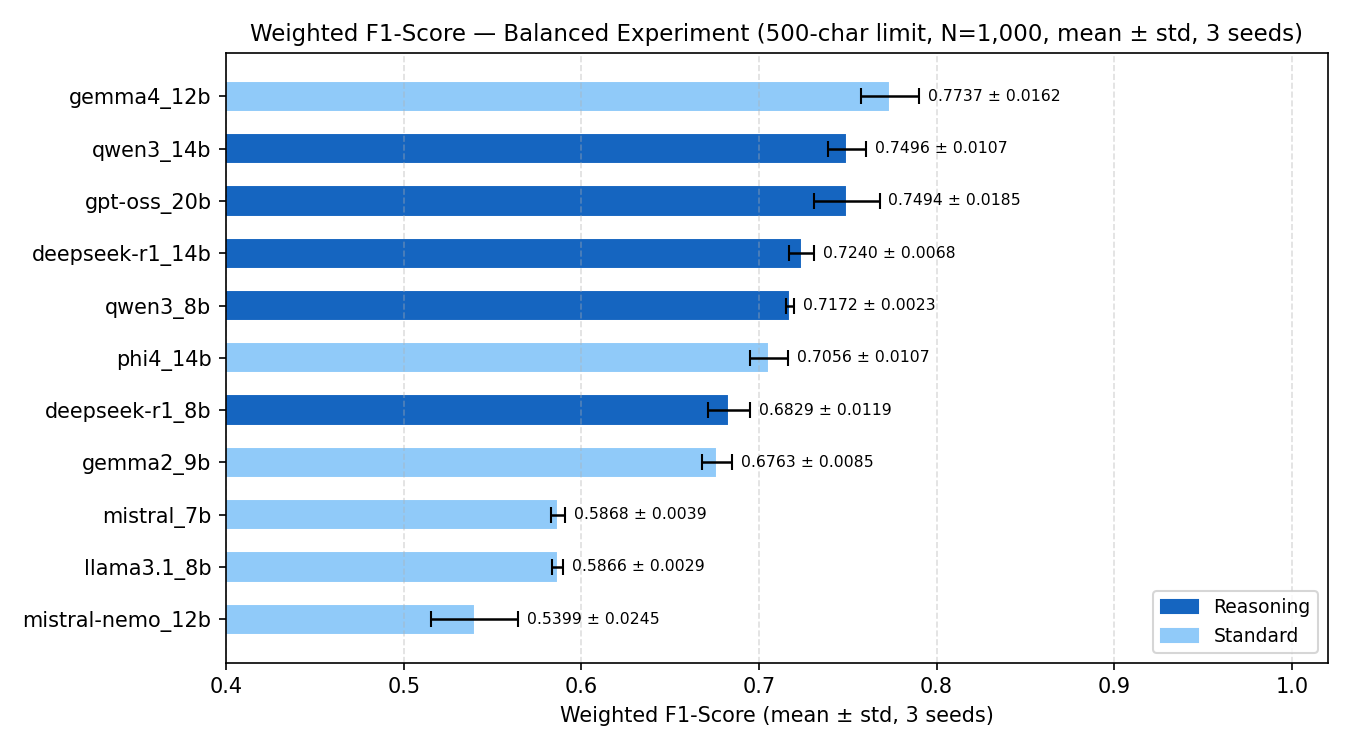
\includegraphics[width=0.82\textwidth]{figures/v2/f1_balanced_errbar.png}
  \caption{Weighted F1-scores for all eleven models in Experiment~A (Balanced),
           shown as mean~$\pm$~std over three seeds.
           Reasoning models are shown in dark blue; standard models in
           light blue. \texttt{gemma4:12b} (standard) leads all reasoning models.}
  \label{fig:f1_bar}
\end{figure*}

\begin{figure*}[t]
  \centering
  \begin{minipage}[b]{0.31\textwidth}
    \centering
    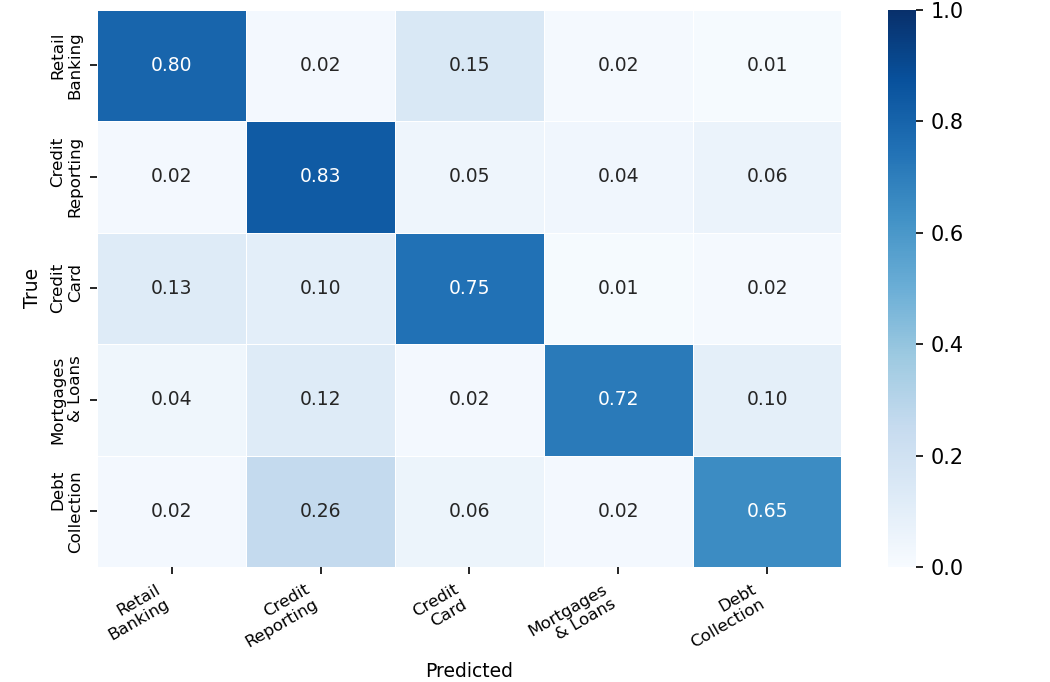
\includegraphics[width=\linewidth]{figures/v2/confusion_gpt-oss_20b_balanced.png}
    \par\smallskip
    {\footnotesize (a)~\texttt{gpt-oss:20b}}
  \end{minipage}
  \hfill
  \begin{minipage}[b]{0.31\textwidth}
    \centering
    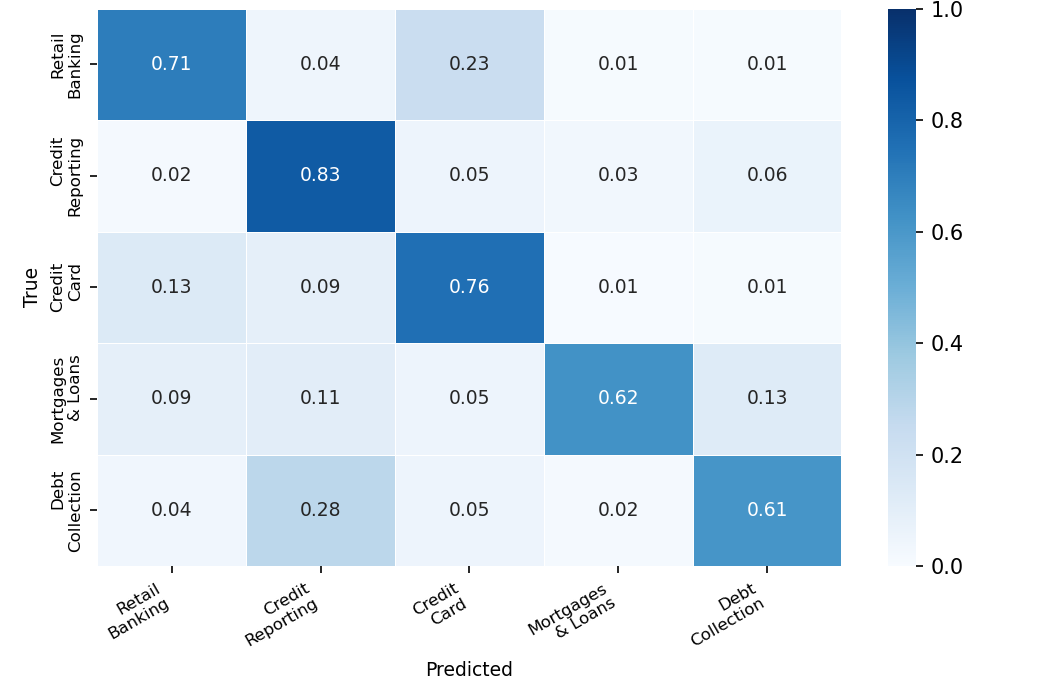
\includegraphics[width=\linewidth]{figures/v2/confusion_phi4_14b_balanced.png}
    \par\smallskip
    {\footnotesize (b)~\texttt{phi4:14b}}
  \end{minipage}
  \hfill
  \begin{minipage}[b]{0.31\textwidth}
    \centering
    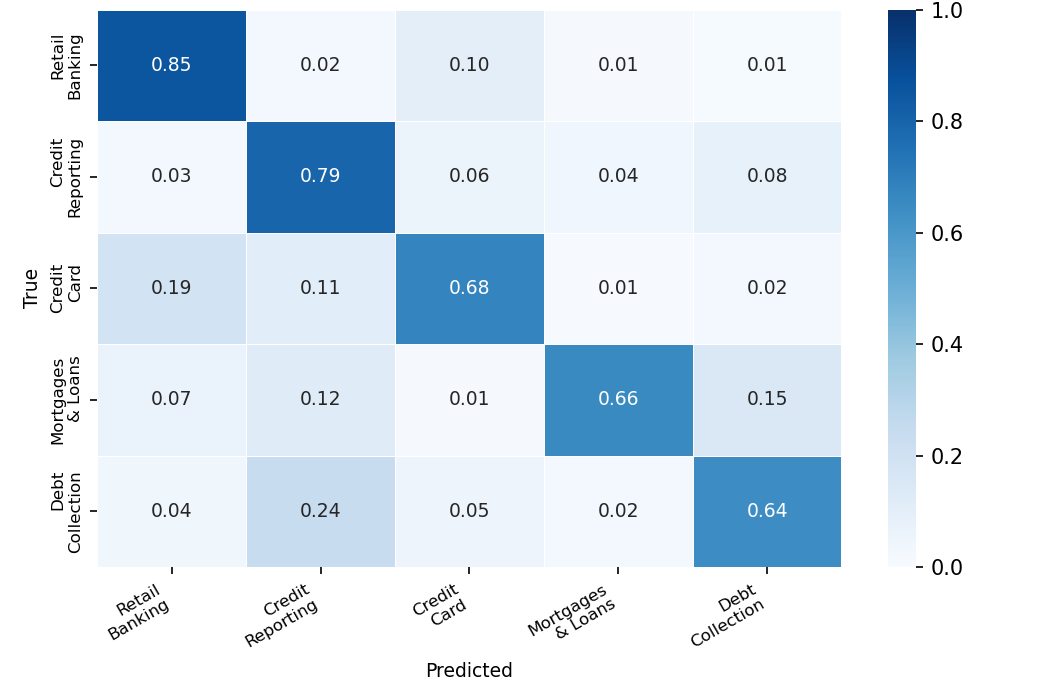
\includegraphics[width=\linewidth]{figures/v2/confusion_deepseek-r1_14b_balanced.png}
    \par\smallskip
    {\footnotesize (c)~\texttt{deepseek-r1:14b}}
  \end{minipage}
  \caption{Averaged confusion matrices for selected models (Experiment~A, $N{=}1{,}000$,
           mean over 3~seeds). Rows: true labels; columns: predicted labels.
           (a)~\texttt{gpt-oss:20b}: top reasoning model, handles \texttt{credit\_reporting}
           and \texttt{retail\_banking} well with some confusion between
           \texttt{mortgages\_and\_loans} and \texttt{credit\_card}.
           (b)~\texttt{phi4:14b}: best sub-1-second standard model, strong diagonal with
           minor confusion.
           (c)~\texttt{deepseek-r1:14b}: second reasoning model, near-zero off-label rate;
           main confusions between \texttt{credit\_card} and \texttt{mortgages\_and\_loans}.}
  \label{fig:conf_all}
\end{figure*}

\subsection{Experiment B: Imbalanced Evaluation}

Table~\ref{tab:results_imbalanced} presents results for Experiment~B,
again as means over three seeds. All eleven models show numerically
higher accuracy and F1 compared to Experiment~A.
\texttt{gpt-oss:20b} regains the top position under imbalanced conditions,
with mean accuracy $0.782 \pm 0.017$ and F1 $0.783 \pm 0.016$.
\texttt{gemma4:12b} follows closely in second place
(Acc~$0.776 \pm 0.015$, F1~$0.779 \pm 0.014$), and
\texttt{qwen3:14b} ranks third (F1~$0.772 \pm 0.013$).
The top five models (\texttt{gpt-oss:20b}, \texttt{gemma4:12b},
\texttt{qwen3:14b}, \texttt{qwen3:8b}, \texttt{phi4:14b}) all achieve
weighted F1 $\geq 0.754$. The imbalanced setting changes the absolute
score level more than the identity of the leading models. However,
the gains for \texttt{llama3.1:8b} and \texttt{mistral:7b} should not
be interpreted as genuine robustness improvements, because both models
still produce many off-label outputs and benefit from the dominant
\texttt{credit\_reporting} class.

\begin{table*}[!t]
  \renewcommand{\arraystretch}{1.2}
  \caption{Experiment B Results --- Imbalanced ($N = 1{,}000$, mean of 3 seeds; std in parentheses)}
  \label{tab:results_imbalanced}
  \centering
  \scriptsize
  \setlength{\tabcolsep}{4pt}
  \begin{tabular}{@{}llrrrrc@{}}
    \toprule
    \textbf{Model} & \textbf{Type} & \textbf{Acc.} & \textbf{F1$_w$} & \textbf{F1$_m$} & \textbf{Lat.(s)} & \textbf{Off-label} \\
    \midrule
    \texttt{gpt-oss:20b}      & Reasoning & 0.782\,({\footnotesize$\pm$.017}) & 0.783\,({\footnotesize$\pm$.016}) & 0.740 &  4.01 & 0.0 \\
    \texttt{gemma4:12b}       & Standard  & 0.776\,({\footnotesize$\pm$.015}) & 0.779\,({\footnotesize$\pm$.014}) & 0.741 & 10.61 & 2.7 \\
    \texttt{qwen3:14b}        & Reasoning & 0.772\,({\footnotesize$\pm$.012}) & 0.772\,({\footnotesize$\pm$.013}) & 0.730 &  5.53 & 0.0 \\
    \texttt{qwen3:8b}         & Reasoning & 0.766\,({\footnotesize$\pm$.008}) & 0.762\,({\footnotesize$\pm$.007}) & 0.719 &  6.97 & 0.3 \\
    \texttt{phi4:14b}         & Standard  & 0.753\,({\footnotesize$\pm$.004}) & 0.754\,({\footnotesize$\pm$.002}) & 0.696 &  0.58 & 0.0 \\
    \texttt{deepseek-r1:14b}  & Reasoning & 0.746\,({\footnotesize$\pm$.017}) & 0.748\,({\footnotesize$\pm$.015}) & 0.700 &  7.32 & 0.3 \\
    \texttt{deepseek-r1:8b}   & Reasoning & 0.738\,({\footnotesize$\pm$.012}) & 0.731\,({\footnotesize$\pm$.011}) & 0.677 &  4.46 & 2.3 \\
    \texttt{gemma2:9b}        & Standard  & 0.720\,({\footnotesize$\pm$.012}) & 0.719\,({\footnotesize$\pm$.014}) & 0.656 &  0.67 & 0.3 \\
    \texttt{mistral-nemo:12b} & Standard  & 0.653\,({\footnotesize$\pm$.011}) & 0.641\,({\footnotesize$\pm$.013}) & 0.538 &  0.59 & 0.7 \\
    \texttt{mistral:7b}       & Standard  & 0.649\,({\footnotesize$\pm$.010}) & 0.661\,({\footnotesize$\pm$.010}) & 0.566 &  0.23 & 42.3 \\
    \texttt{llama3.1:8b}      & Standard  & 0.632\,({\footnotesize$\pm$.006}) & 0.647\,({\footnotesize$\pm$.012}) & 0.564 &  0.56 & 57.3 \\
    \bottomrule
    \multicolumn{7}{l}{\footnotesize F1$_w$: weighted F1; F1$_m$: macro F1; Lat.: mean latency per prediction.}
  \end{tabular}
\end{table*}

The relative model ranking is broadly preserved compared to
Experiment~A, with one notable reordering: \texttt{gpt-oss:20b}
reclaims the top position while \texttt{gemma4:12b} drops to second.
The macro-F1 column makes the imbalance effect visible:
\texttt{gpt-oss:20b} has weighted F1~0.783 but macro-F1~0.740, while
\texttt{llama3.1:8b} has weighted F1~0.647 but macro-F1~0.564.
The gap shows that weighted metrics substantially overstate
minority-class performance in the imbalanced setting.
The F1-score distribution mirrors Experiment~A in its broad ordering
(Fig.~\ref{fig:comparison_ab} right bars), with \texttt{gpt-oss:20b},
\texttt{gemma4:12b}, and \texttt{qwen3:14b} forming the leading group.

\subsection{Cross-Experiment Comparison}

Fig.~\ref{fig:comparison_ab} provides a side-by-side view of accuracy
across both experiments. All models improve numerically from
Experiment~A to Experiment~B; the shift is most pronounced for
\texttt{mistral:7b} ($\Delta$acc~$= +0.055$)
and \texttt{llama3.1:8b} ($\Delta$acc~$= +0.054$), the two models with the
highest off-label counts. This pattern suggests that under imbalanced
conditions, a model defaulting to the majority class can still achieve
a deceptively high aggregate score. \texttt{mistral-nemo:12b} improves
by $+0.094$ accuracy from Experiment~A to B, the largest gain of all
eleven models, further confirming that its Experiment~A result reflects
failure to maintain the balanced classification task rather than a
model-quality ceiling.

\begin{figure*}[t]
  \centering
  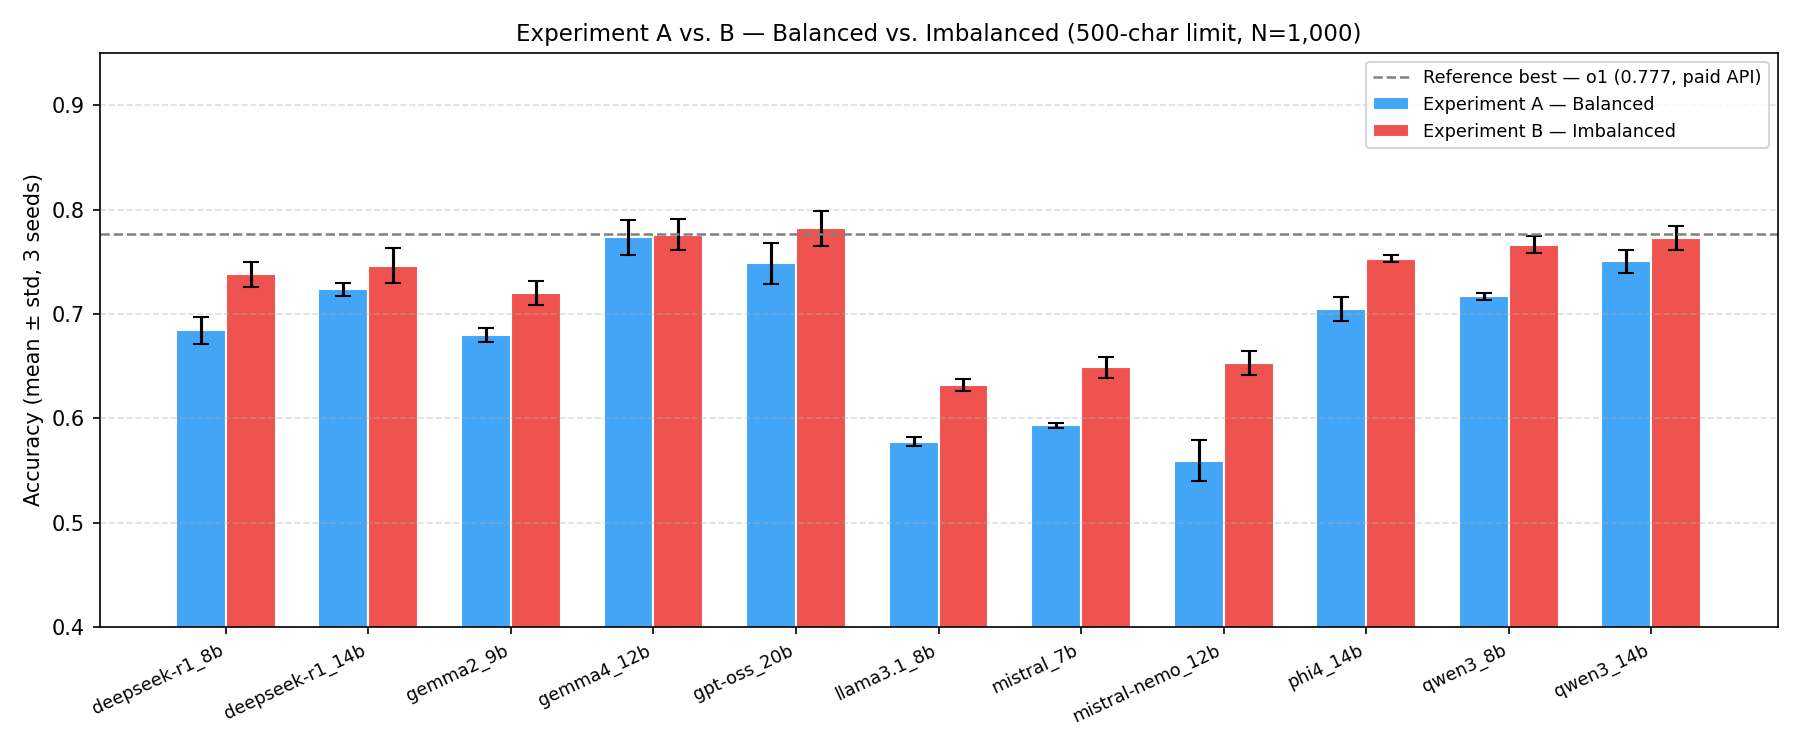
\includegraphics[width=0.85\textwidth]{figures/v2/comparison_A_vs_B.png}
  \caption{Side-by-side comparison of accuracy (mean~$\pm$~std, 3 seeds)
           across Experiment~A (Balanced, blue) and Experiment~B
           (Imbalanced, red) for all models ($N{=}1{,}000$). The dashed
           reference line marks the best published paid-API result
           (o1, 0.777). The upward shift in Experiment~B partially
           reflects class imbalance rather than genuine model improvement.}
  \label{fig:comparison_ab}
\end{figure*}

\subsection{Comparison with Paid-API Baselines}

Fig.~\ref{fig:vs_reference} compares all eleven of our open-source
models with the five best reported results from Roumeliotis~et~al.\
\cite{roumeliotis2025think}. Table~\ref{tab:vs_reference} summarises
the key comparison points. Our best model, \texttt{gemma4:12b},
achieves a mean accuracy of $0.774 \pm 0.017$ and F1 of $0.774 \pm 0.016$
--- achieving performance competitive with the paid GPT-4.5 (F1~0.7763)
and o1 (F1~0.7764) under the matched evaluation protocol, with no
commercial API expenditure. Our results indicate that a freely
available, locally-deployed 12B standard model can achieve performance
competitive with the two most capable paid reasoning models reported
in the literature.
\texttt{qwen3:14b} (F1~$0.750$) and \texttt{gpt-oss:20b} (F1~$0.749$)
both exceed the paid GPT-4o baseline (0.7358), although they remain
below Claude~3.7 Sonnet (F1~0.7626).
All eleven open-source models in this study were evaluated on the
\emph{exact same} complaint instances (fixed NumPy seeds, identical
draws for every model), so every within-study comparison is
instance-identical. The cross-paper comparison with GPT-4.5 and o1
results from Roumeliotis~et~al.\ \cite{roumeliotis2025think} is
protocol-matched rather than instance-paired, since that paper does
not publish its sampled complaint identifiers.
The cost differential is stark: the reference paper reported
o1 costs of \$24.24 per thousand predictions, versus no commercial
API expenditure for all our models.

\begin{table*}[!t]
  \renewcommand{\arraystretch}{1.2}
  \caption{Zero-Shot Performance vs.\ API Cost (Balanced, $N{=}1{,}000$).
           Commercial API figures are from \cite{roumeliotis2025think}.
           $^\dagger$No commercial API expenditure; compute costs are borne
           by institutional HPC allocation (TRUBA ARF).}
  \label{tab:vs_reference}
  \centering
  \scriptsize
  \setlength{\tabcolsep}{5pt}
  \begin{tabular}{@{}llrrl@{}}
    \toprule
    \textbf{Model} & \textbf{Source} & \textbf{Accuracy} & \textbf{F1} & \textbf{API Cost/1k} \\
    \midrule
    o1                           & Paid API     & 0.777             & 0.7764            & \$24.24 \\
    GPT-4.5                      & Paid API     & 0.774             & 0.7763            & \$12.32 \\
    \textbf{\texttt{gemma4:12b}} & \textbf{Open-source} & $\mathbf{0.774{\pm}.017}$ & $\mathbf{0.774{\pm}.016}$ & \textbf{none}$^\dagger$ \\
    Claude~3.7~Sonnet            & Paid API     & 0.765             & 0.7626            & \$0.64  \\
    Gemini~2.0~Flash             & Paid API     & 0.758             & 0.7586            & \$0.04  \\
    \texttt{qwen3:14b}           & Open-source  & $0.751{\pm}.011$  & $0.750{\pm}.011$  & none$^\dagger$  \\
    \texttt{gpt-oss:20b}         & Open-source  & $0.748{\pm}.020$  & $0.749{\pm}.019$  & none$^\dagger$  \\
    GPT-4o                       & Paid API     & 0.736             & 0.7358            & \$0.45  \\
    \texttt{deepseek-r1:14b}     & Open-source  & $0.724{\pm}.006$  & $0.724{\pm}.007$  & none$^\dagger$  \\
    \texttt{qwen3:8b}            & Open-source  & $0.717{\pm}.003$  & $0.717{\pm}.002$  & none$^\dagger$  \\
    \texttt{phi4:14b}            & Open-source  & $0.705{\pm}.012$  & $0.706{\pm}.011$  & none$^\dagger$  \\
    \bottomrule
  \end{tabular}
\end{table*}

\begin{figure*}[t]
  \centering
  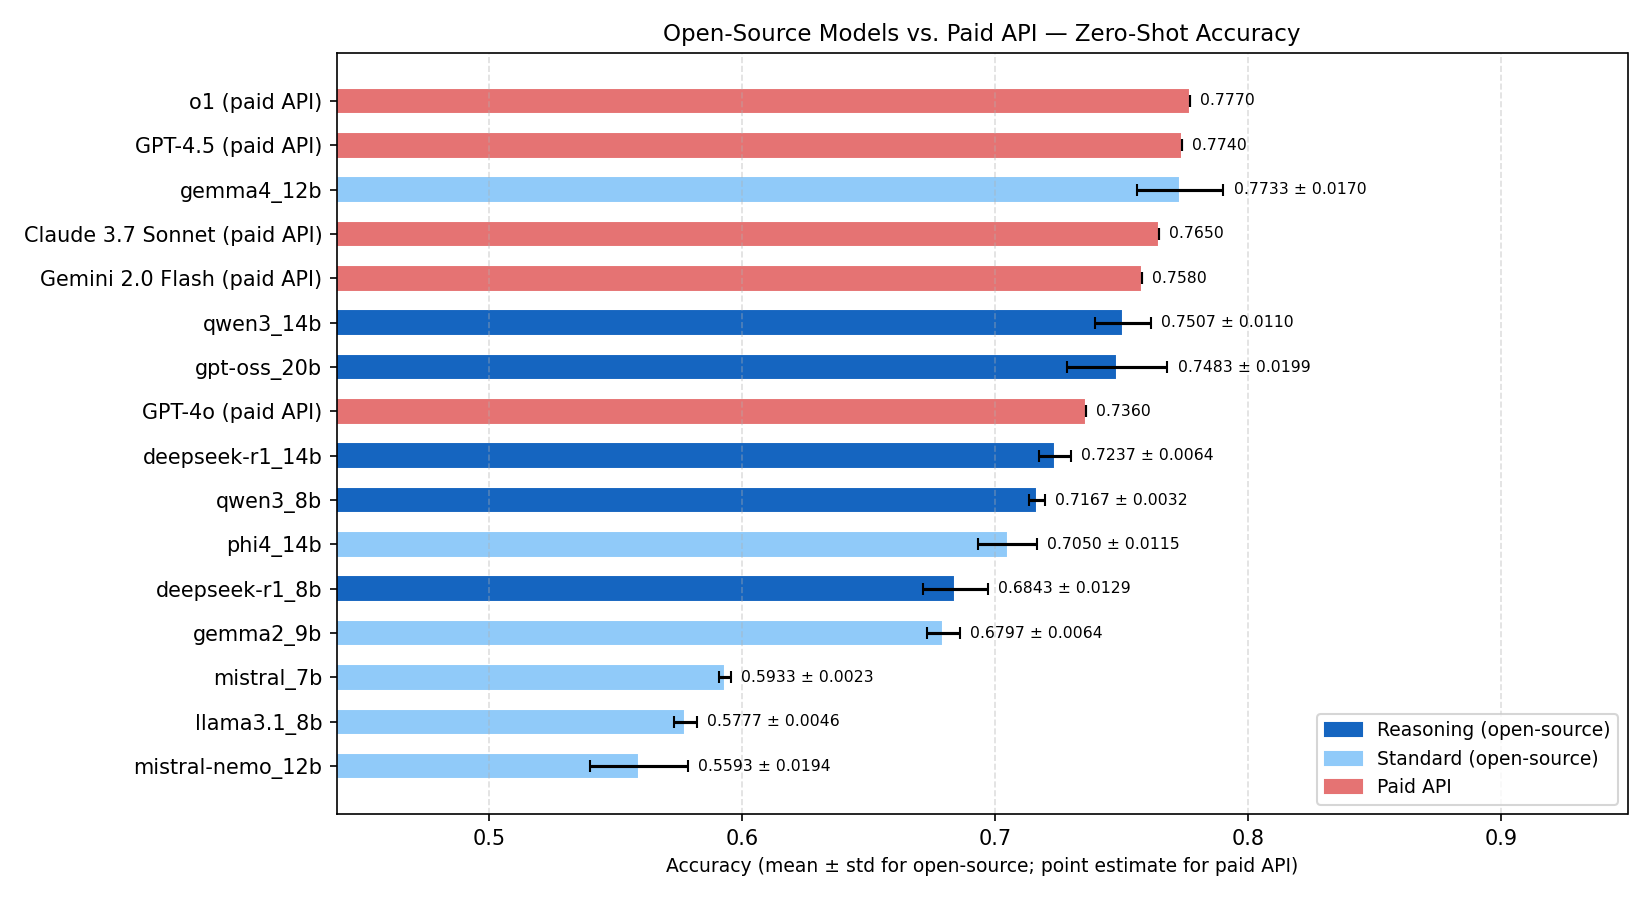
\includegraphics[width=0.82\textwidth]{figures/v2/vs_reference.png}
  \caption{Accuracy of all eleven open-source models (Experiment~A,
           mean~$\pm$~std over 3 seeds) alongside five paid-API baselines
           from \cite{roumeliotis2025think}.
           \texttt{gemma4:12b} achieves performance comparable to GPT-4.5 and o1 under the protocol-matched setting, with no commercial API expenditure.
           Open-source error bars reflect seed variability; paid-API
           figures are single-run point estimates.}
  \label{fig:vs_reference}
\end{figure*}

\subsection{Narrative Length Sensitivity}
\label{sec:sensitivity}

Fig.~\ref{fig:size_sensitivity} compares mean accuracy on
250-character-limit versus 500-character-limit narratives for the
balanced condition (both at $N{=}1{,}000$). The overall ranking
is highly stable: no model changes its relative rank by more than
one position between the two length limits. Most models improve by
0--3 percentage points moving from shorter to longer narratives, with
\texttt{deepseek-r1:14b} (+1.6~pp) and \texttt{llama3.1:8b} (+2.8~pp)
showing the largest gains, suggesting these models benefit from the
additional context available in longer narratives.
\texttt{gpt-oss:20b} and \texttt{mistral-nemo:12b} show virtually no
change ($\leq$0.1~pp), indicating that their behaviour is not sensitive
to narrative length in this range. The stability of the top-cluster
ranking confirms that the 500-character results represent genuine
model-quality differences and not length-specific artefacts.

\begin{figure*}[t]
  \centering
  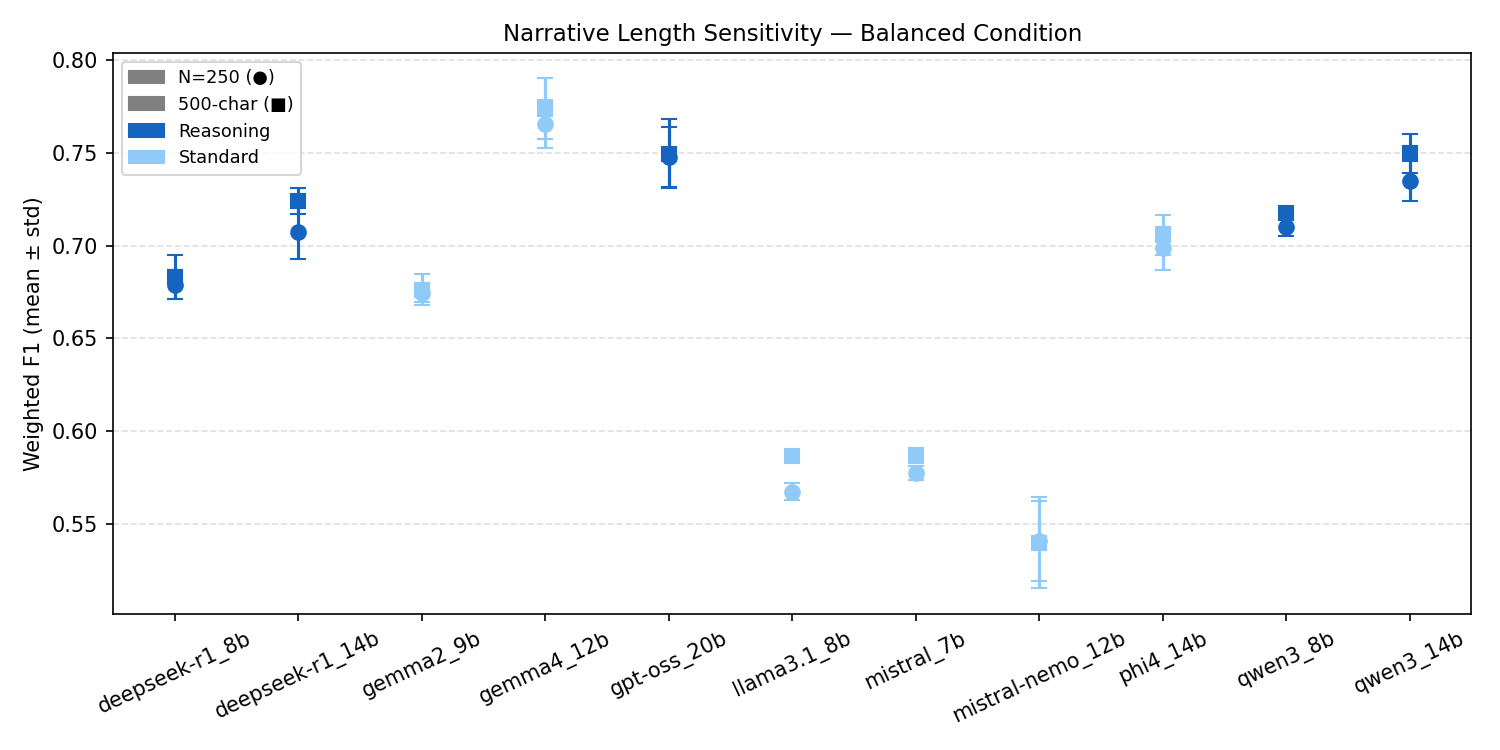
\includegraphics[width=0.82\textwidth]{figures/v2/size_sensitivity_balanced.png}
  \caption{Mean accuracy on 250-char vs 500-char narrative variants
           (Balanced, $N{=}1{,}000$, 3~seeds) for all eleven models.
           Rankings are highly stable; most models show small gains
           with longer narratives.}
  \label{fig:size_sensitivity}
\end{figure*}

\subsection{Latency Analysis}

Mean per-prediction latency is shown in the Lat.(s) column of
Tables~\ref{tab:results_balanced} and~\ref{tab:results_imbalanced}.
Standard models are notably faster: \texttt{mistral:7b} completes
a prediction in 0.23~s on average, while \texttt{phi4:14b} requires
only 0.54~s despite being twice the parameter count. Reasoning models
are slower: \texttt{deepseek-r1:14b} takes 9.33~s per prediction due
to its chain-of-thought trace. \texttt{gemma4:12b}, despite being a
standard model, has the highest latency at 17.1~s --- attributable to
its longer response patterns rather than chain-of-thought. The
latency--accuracy trade-off is model-type dependent: \texttt{phi4:14b}
achieves the best latency-accuracy ratio among all models (0.54~s,
F1~0.706). Fig.~\ref{fig:latency} shows the F1-score distribution
across all eleven models in Experiment~B, providing a visual complement
to Table~\ref{tab:results_imbalanced}.

\begin{figure*}[t]
  \centering
  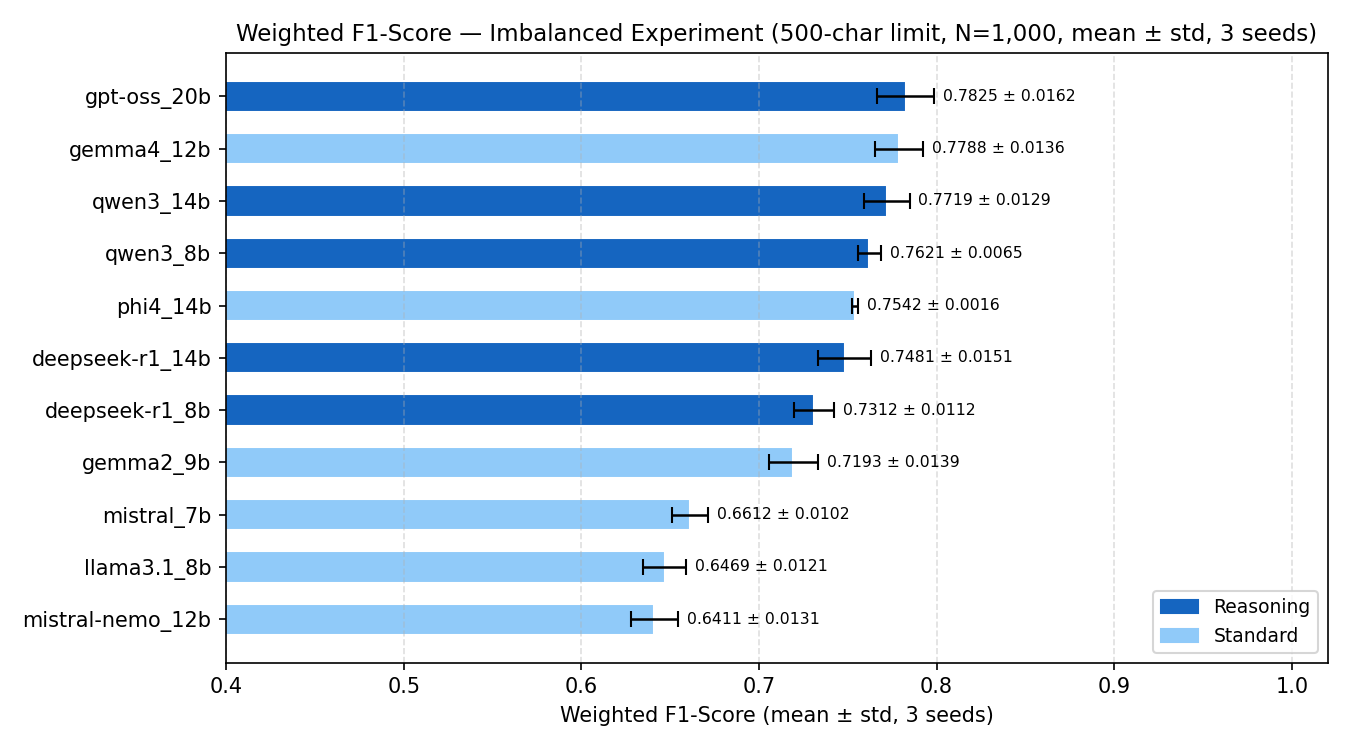
\includegraphics[width=0.82\textwidth]{figures/v2/f1_imbalanced_errbar.png}
  \caption{Weighted F1-scores for all eleven models in Experiment~B
           (Imbalanced), shown as mean~$\pm$~std over three seeds,
           with \texttt{gpt-oss:20b} at the top and \texttt{gemma4:12b}
           a close second.}
  \label{fig:latency}
\end{figure*}

\subsection{Per-Class Breakdown for Leading Models}
\label{sec:per_class_metrics}

Table~\ref{tab:per_class} reports per-class F1 for the three leading
models in each experiment, confirming that aggregate weighted F1 masks
important minority-class variation. In Experiment~B all three models
jump to ${\geq}0.84$ F1 on \texttt{credit\_reporting} while minority
classes remain in the 0.65--0.77 range, confirming the majority-class
bias effect discussed in Section~\ref{sec:discussion}.

\begin{table*}[b]
  \renewcommand{\arraystretch}{1.2}
  \caption{Per-Class F1 for Leading Models (Exp.~A and~B, $N{=}1{,}000$)}
  \label{tab:per_class}
  \centering
  \scriptsize
  \setlength{\tabcolsep}{5pt}
  \begin{tabular}{@{}llccccc@{}}
    \toprule
    \textbf{Exp.} & \textbf{Model} &
    \textbf{Retail} &
    \textbf{CreditRep.} &
    \textbf{Card} &
    \textbf{Mortg.} &
    \textbf{Debt} \\
    \midrule
    A & \texttt{gemma4:12b}      & 0.8247 & 0.7432 & 0.7634 & 0.8194 & 0.7178 \\
    A & \texttt{qwen3:14b}       & 0.7855 & 0.7212 & 0.7296 & 0.8097 & 0.7019 \\
    A & \texttt{gpt-oss:20b}     & 0.7939 & 0.7137 & 0.7394 & 0.7953 & 0.7045 \\
    \midrule
    B & \texttt{gpt-oss:20b}     & 0.7508 & 0.8527 & 0.6657 & 0.7404 & 0.6919 \\
    B & \texttt{gemma4:12b}      & 0.7676 & 0.8453 & 0.6719 & 0.7442 & 0.6769 \\
    B & \texttt{qwen3:14b}       & 0.7353 & 0.8437 & 0.6544 & 0.7427 & 0.6727 \\
    \bottomrule
    \multicolumn{7}{l}{\footnotesize Mortg. = Mortgages \& Loans.}
  \end{tabular}
\end{table*}


% =============================================================
\section{Discussion}
\label{sec:discussion}

\subsection{Reasoning vs.\ Standard Models}

The most notable finding across both experiments is that model
\emph{generation} and \emph{architecture quality} can outweigh model
type (reasoning vs.\ standard). \texttt{gemma4:12b}, a standard
non-reasoning model, achieves the highest weighted F1 in
Experiment~A ($0.774 \pm 0.016$), surpassing all five reasoning models
including \texttt{gpt-oss:20b} (F1~$0.749$), which has 67\,\% more
parameters. This challenges the simple hypothesis that reasoning models
are necessary for structured zero-shot classification tasks.

That said, a nuanced pattern emerges when scale is controlled.
At the 8B tier, reasoning models (\texttt{deepseek-r1:8b},
\texttt{qwen3:8b}) generally outperform standard models of similar
size (\texttt{gemma2:9b}, \texttt{llama3.1:8b}, \texttt{mistral:7b}).
At the 14B tier, \texttt{qwen3:14b} (Reasoning, F1~0.750) and
\texttt{phi4:14b} (Standard, F1~0.706) are both strong, but the
reasoning advantage is narrower. The 12B result from \texttt{gemma4:12b}
suggests that the latest-generation standard models have closed the
reasoning gap through improved alignment and instruction-following
training, consistent with the broader evidence that chain-of-thought
benefits diminish as standard-model quality improves
\cite{wei2022chainofthought,guo2025deepseekr1}.

An unexpected finding is the underperformance of \texttt{mistral-nemo:12b}
(F1~$0.540 \pm 0.025$ in Experiment~A, rank~11 of~11), which falls
below both its smaller sibling \texttt{mistral:7b} (F1~$0.587$) and
all other 12B-tier models. Its off-label rate is low (0.7 per run),
indicating that the model does produce parseable JSON but assigns
incorrect categories. This suggests that the Mistral Nemo architecture,
while competitive in general-purpose tasks, does not transfer as
effectively to this narrow structured classification setting.

\subsection{Within-Family Performance Patterns}

The expanded eleven-model set allows direct within-family comparisons
that were not possible in the original eight-model design.

\textbf{Gemma family (Google):} \texttt{gemma4:12b} (F1~0.774)
outperforms \texttt{gemma2:9b} (F1~0.676) by 0.098 F1 points ---
the largest within-family gain observed. This improvement is driven by
stronger category disambiguation.
Off-label counts increase slightly from gemma2 (mean 0.3) to
gemma4 (mean 3.7), but gemma4's rare off-label cases are
classification mismatches rather than format failures ---
a qualitatively different error mode that is less disruptive
to downstream parsing. The generation gap (Gemma~2 to
Gemma~4) is more impactful than the parameter gap (9B to 12B),
confirming that training recipe and alignment improvements can
outweigh raw scale.

\textbf{Mistral family (Mistral AI):} \texttt{mistral-nemo:12b}
(F1~0.540) performs \emph{worse} than \texttt{mistral:7b} (F1~0.587)
in Experiment~A, despite having 71\,\% more parameters. Their
error modes are opposite: \texttt{mistral:7b} frequently produces
off-label outputs (58.7 per run), whereas \texttt{mistral-nemo:12b}
commits to valid categories but assigns them incorrectly.
Latency is comparable (0.23~s vs 0.59~s). This suggests that Mistral
Nemo's training optimised for different task types and that the
12B Nemo architecture does not generalise as well as Mistral~7B to
tightly constrained JSON classification.

\textbf{Qwen3 family (Alibaba):} \texttt{qwen3:14b} (F1~0.750)
outperforms \texttt{qwen3:8b} (F1~0.717) consistently across both
experiments, with no off-label predictions in either case. The
+0.033 F1 gain is achieved with comparable latency (5.73~s vs 5.19~s),
making \texttt{qwen3:14b} the better choice when additional VRAM is
available (9.3~GB vs 5.2~GB). Both models demonstrate that the Qwen3
architecture transfers well to structured zero-shot tasks.

\textbf{DeepSeek-R1 family (DeepSeek):} \texttt{deepseek-r1:14b}
(F1~0.724) outperforms \texttt{deepseek-r1:8b} (F1~0.683) by 0.041
F1 points. Off-label counts also improve with scale (1.3 vs 2.0).
Latency increases proportionally (9.33~s vs 5.14~s), reflecting
the longer reasoning traces generated by the larger model. The
performance gap is consistent across all three seeds, confirming
that scale reliably improves the DeepSeek-R1 distillation quality.

\subsection{Off-Label Prediction Behaviour}

Off-label predictions --- responses where the model returned a label
not in the prescribed five categories --- are a direct measure of
instruction-following reliability. The two models with the highest
off-label counts in Experiment~A
(\texttt{llama3.1:8b}:~67; \texttt{mistral:7b}:~59)
also rank among the lowest in F1. This is
not coincidental: off-label responses are counted as prediction
errors, directly reducing accuracy and recall. In Experiment~A, the
reasoning models are generally more disciplined than the weakest
standard models: \texttt{qwen3:14b}, \texttt{gpt-oss:20b}, and
\texttt{qwen3:8b} produce zero off-label predictions, while
\texttt{deepseek-r1:14b} and \texttt{deepseek-r1:8b} remain low at
1.3 and 2.0 off-label predictions per run, respectively.
The better instruction-following of reasoning models reflects the
structured nature of chain-of-thought: the model explicitly reasons
about which label is appropriate before formatting its output,
reducing the likelihood of hallucinating a novel category.

The raw status logs show that off-label behaviour has two distinct
forms. \texttt{llama3.1:8b} primarily fails at the formatting/parsing
level, producing a mean of 67 parse errors in Experiment~A and 57 in
Experiment~B. In contrast, \texttt{mistral:7b} usually returns
parseable JSON but invents labels outside the allowed taxonomy,
producing a mean of 59 valid-but-out-of-vocabulary labels in
Experiment~A and 42 in Experiment~B. Smaller counts for \texttt{phi4:14b},
\texttt{gemma2:9b}, and \texttt{deepseek-r1:8b} are also
valid-but-out-of-vocabulary labels such as \texttt{unknown} or
\texttt{health\_insurance}. This distinction matters operationally:
parse errors indicate output-format failure, whereas out-of-vocabulary
labels indicate failure to stay within the regulatory taxonomy.

Off-label behaviour should therefore be interpreted not only as an
accuracy penalty but also as an operational reliability signal. In a
regulated complaint-routing pipeline, an invented category such as
\texttt{unknown}, \texttt{loan}, or \texttt{credit\_dispute} may be
more disruptive than an ordinary within-taxonomy misclassification,
because downstream systems typically assume that every prediction
belongs to the fixed regulatory label set. The observed difference
between parse errors and valid-but-out-of-taxonomy labels suggests
that local LLM evaluations should report output discipline separately
from classification quality, especially when models are intended for
semi-automated banking, compliance, or regulator-facing workflows.

Notably, the off-label count for \texttt{mistral:7b} improves
substantially in Experiment~B (from 59 to 42), suggesting that the
dominant \texttt{credit\_reporting} class provides an easier default
that is more likely to receive a correctly-formatted taxonomy label.
By contrast, \texttt{llama3.1:8b} remains unreliable
(67 in Experiment~A vs 57 in Experiment~B), indicating that its
parsing failures are not resolved by class imbalance alone.

\subsection{Latency--Accuracy Trade-off}

From a practical deployment perspective, the latency results present
an important consideration. The fastest model, \texttt{mistral:7b}
(0.23~s), achieves only F1~0.587 --- far below the leading models in
Experiment~A.
\texttt{phi4:14b}, at 0.54~s per prediction and F1~0.706, offers
the most favourable accuracy-to-latency ratio of any model tested.
For applications requiring both real-time response and reasonable
accuracy, \texttt{phi4:14b} is the recommended choice.

Reasoning models are consistently slower: \texttt{deepseek-r1:14b}
takes 9.33~s per prediction on average across seeds and nodes.
At 500 predictions, this translates to roughly 1.3~hours of total
inference time on a single V100. For
large-scale regulatory applications processing millions of complaints,
the time budget would need to be considered alongside model quality.
All reported latency figures for reasoning models include the full
chain-of-thought generation trace; the final JSON label is extracted
from the end of this trace via the regex described in
Section~\ref{sec:setup}. Latency comparisons between reasoning and
standard models should therefore be interpreted as end-to-end
wall-clock cost rather than pure decoding speed.

\subsection{Deployment Recommendations}

Based on the combined latency and accuracy evidence, we offer the
following concrete deployment recommendations for practitioners.

\textbf{Maximum accuracy (offline / batch):}
Use \texttt{gemma4:12b}. It achieves the highest balanced F1 (0.774),
competitive with paid frontier APIs at no commercial API cost, and requires 7.6~GB VRAM.
Latency of 17.1~s per prediction is acceptable for batch triage of
large complaint archives.

\textbf{Real-time deployment ($<$1\,s latency required):}
Use \texttt{phi4:14b}. It offers F1~0.706 at just 0.54~s per
prediction --- the best accuracy-to-latency ratio among all eleven models.
At roughly 110~predictions per minute throughput, it can serve a
moderate complaint routing queue in real-time on a single V100.

\textbf{Constrained VRAM ($\leq$5.5\,GB):}
Use \texttt{qwen3:8b} (5.2~GB, F1~0.717, 5.19~s). It produces zero
off-label predictions and outperforms all other sub-6\,GB models.

\textbf{Avoid} \texttt{mistral:7b} and \texttt{llama3.1:8b} in
zero-shot settings: both produce $>$50 off-label predictions per
1,000 samples on average, making them operationally unreliable
without post-processing.
\texttt{mistral-nemo:12b} is also not recommended for this task
despite its size advantage.

Taken together, these recommendations translate into concrete
advantages that go beyond cost. At moderate scale (one million
complaints per year), deploying \texttt{gemma4:12b} instead of the
best-performing paid API model would avoid roughly \$12,320 in API
fees with no measurable quality loss. More importantly for regulated
institutions, local deployment eliminates the need to transmit
sensitive financial complaint narratives to any third-party service
--- a requirement that may be mandatory under data-governance
frameworks such as GDPR, the EU AI Act, or national banking secrecy
rules. \texttt{qwen3:14b} and \texttt{gpt-oss:20b} similarly exceed
the paid GPT-4o baseline (F1~0.7358) at zero API cost. This should
not be read as computation being free: local inference still consumes
GPU time, electricity, and institutional HPC capacity. The practical
gain is the simultaneous elimination of recurring API charges,
third-party data transfer obligations, and vendor lock-in --- all
of which are material concerns in compliant financial deployments.

\subsection{Interpreting the Imbalanced Results}

The across-the-board increase in accuracy and F1 from Experiment~A
to Experiment~B demands careful interpretation. While a genuine
improvement is possible --- models may be aided by the greater
frequency of \texttt{credit\_reporting} training signal in
their pre-training corpora, which coincides with its frequency in
the CFPB data --- a more parsimonious explanation exists:
\emph{class imbalance inflates aggregate accuracy metrics}.

When 51.1\,\% of the test set belongs to a single class, a model
that classifies most ambiguous narratives as \texttt{credit\_reporting}
will achieve a high weighted accuracy even if its per-class performance
is poor. The particularly pronounced gains for \texttt{llama3.1:8b}
(+4.2~pp accuracy) and \texttt{mistral:7b} (+5.5~pp accuracy) --- the
two highest off-label producers in Experiment~A --- are consistent
with this mechanism: under imbalanced conditions, a confused model
benefits disproportionately from majority-class guesses. We therefore
caution against using Experiment~B accuracy as a simple indicator of
model quality and recommend that future evaluations report per-class
precision and recall alongside aggregate metrics.

\subsection{Limitations}

This study has several limitations. First, while all eleven models
in this study share \emph{identical} test instances (fixed seeds,
same complaint draws for every model), the cross-paper comparison
with GPT-4.5 and o1 results from Roumeliotis~et~al.\
\cite{roumeliotis2025think} is protocol-matched rather than
instance-paired, since the reference paper does not release the
exact sampled complaint identifiers.
Second, the 500-character length filter reduces inference cost but
also shifts the class distribution, especially increasing the share of
\texttt{credit\_reporting}; future work should test whether the same
patterns hold for longer narratives. Third, lowercasing and special-
character removal may discard useful cues such as account-number
patterns, capitalization, dates, or punctuation; the effect of less
aggressive LLM-oriented preprocessing remains untested. Fourth, all
experiments use $N{=}1{,}000$ examples per seed, evaluated at two
narrative character-length limits (250 and 500 characters) across a
five-class taxonomy; larger sample sizes, longer narratives, and richer
taxonomies may reveal additional drift and rarer category confusions.
Fifth, all local models are evaluated with a single zero-shot prompt.
Prompt wording, output-format instructions, few-shot examples, or
self-consistency decoding may change the relative ranking of models,
particularly for smaller standard models with weaker instruction
following. Sixth, all local models are evaluated in their q4 Ollama
quantised form, so the reported scores conflate model family, model
size, and quantisation effects. Seventh, we cannot rule out pre-training
contamination: open-weight models may have encountered CFPB complaints
or derivative datasets during pre-training, although no task-specific
fine-tuning is used in our experiments. Eighth, the reported \$0 cost
refers to API expenditure, not to the full economic cost of GPU
hardware, electricity, or HPC operation. Finally, the main tables
report weighted aggregate metrics; for operational deployment,
macro-F1 and per-class precision/recall should be inspected to avoid
masking poor minority-class performance.

\subsection{Infrastructure Contribution}

A secondary contribution of this work is the documented HPC
deployment pipeline. The combination of SLURM job scheduling,
offline Ollama serving, and a standard-library-only Python inference
script provides a template that can be applied to other NLP
classification tasks on shared research clusters without requiring
pip-installed dependencies on the compute node. This reproducibility
infrastructure lowers the barrier for other researchers to benchmark
local LLMs on domain-specific tasks.


% =============================================================
\section{Conclusion}
\label{sec:conclusion}

We have presented a comprehensive zero-shot benchmark of eleven
open-source large language models on the CFPB consumer financial
complaint classification task, conducted on the TRUBA ARF HPC cluster
with no commercial API expenditure. Our results demonstrate that the
best open-source model, \texttt{gemma4:12b}, achieves a mean weighted
F1 of $0.774 \pm 0.016$ across three independent seeds on the balanced
evaluation --- achieving performance competitive with the paid GPT-4.5
(F1~0.7763) and o1 (F1~0.7764) under a protocol-matched evaluation
setting. The multi-seed design confirms that
this ranking is statistically stable: standard deviations across seeds
are $\leq 0.02$ for all models, and the top cluster
(\texttt{gemma4:12b}, \texttt{qwen3:14b}, \texttt{gpt-oss:20b})
is consistent across all three seeds. Notably, the top-performing
model is a standard (non-reasoning) 12B model, demonstrating that
the latest generation of standard instruction-tuned models can match
or surpass larger reasoning models on structured classification tasks.
The standard model \texttt{phi4:14b} (F1~$0.706 \pm 0.011$)
offers the best latency--accuracy trade-off at 0.54~s per prediction.

Our secondary imbalanced experiment reveals important evaluation
dynamics: aggregate accuracy improvements under imbalanced
conditions are partially attributable to majority-class bias
rather than genuine model improvement, underscoring the need for
per-class reporting in real-world settings.

From a practical standpoint, these findings validate the viability
of self-hosted LLM deployments for financial NLP tasks: institutions
that cannot share sensitive complaint text with third-party API
providers, or that operate under budget constraints, can now achieve
competitive classification quality using open-weight models on
standard GPU hardware.

Future work will explore five directions.
First, a \emph{quantisation sensitivity study} will evaluate all eleven
models at q4, q8, and fp16 precision to determine whether the accuracy
gains from higher numerical precision justify the increased VRAM cost.
Second, a \emph{prompt sensitivity study} will repeat the
balanced and imbalanced evaluations across prompt variants,
reporting confidence intervals and paired significance tests
beyond the multi-seed McNemar analysis presented here.
Third, we will \emph{fine-tune the same eleven open-weight models} on
the CFPB training split and compare their supervised performance against
their zero-shot counterparts reported here. This paired comparison will
quantify the exact cost of removing the annotation requirement and
clarify whether the remaining small gap between local models and
frontier paid APIs can be closed by task-specific supervised training.
Fourth, \emph{long-narrative robustness} will be examined by relaxing
the 500-character filter and measuring whether additional complaint
context improves classification or instead increases prompt length and
latency costs.
Fifth, the benchmark will be \emph{extended to the full multi-year
CFPB corpus} with a richer category taxonomy to assess scalability
and temporal robustness of the open-source inference pipeline.


% ---- Declarations -------------------------------------------
\section*{Declaration of Competing Interest}
The authors declare that they have no competing interests.

\section*{Funding}
This research received no external funding.

\section*{Acknowledgements}
The numerical calculations reported in this paper were fully performed
at T{\"U}B\.{I}TAK ULAKB\.{I}M, High Performance and Grid Computing
Center (TRUBA resources). The authors gratefully acknowledge
T{\"U}B\.{I}TAK ULAKB\.{I}M for providing access to the TRUBA ARF
cluster and the \texttt{akya-cuda} GPU partition used in this study.

\section*{Code Availability}
All source code, preprocessing scripts, and SLURM job files used in
this study are publicly available at:
\url{https://github.com/muhammettan28/ConsumerComplaintwithLLMs}

% ---- CRediT author statement --------------------------------
\printcredits

\FloatBarrier

% ---- References ---------------------------------------------
\bibliographystyle{cas-model2-names}
\bibliography{references}

\end{document}
